\subsection{Przegląd obiecujących pętli sterowania}

Przedstawiona w poprzedniej sekcji architektura jest jedynie funkcjonalna i zawiera w sobie dużo abstrakcji. Ostateczna postać wewnętrznej zamkniętej pętli sterowania w ENI system jest jeszcze w trakcie specyfikacji. ENI w dokumencie \cite{enioverview} dokonało przeglądu istniejących, możliwych do zaaplikowania architektur zamkniętych pętli sterowania. Niniejsza praca dyplomowa chce zaproponować architekturę do modelowania oraz uruchamiania pętli w ENI System, dlatego ważne jest, aby poznać jej składowe elementy. Nie mamy na celu rozważać dokładnej funkcjonalności tych w środku tych elementów, jedynie poznać ich interfejsy, abyśmy wiedzieli co jako platforma uruchomieniowa powinniśmy być w stanie im zapewnić. 

// Opis wyżej powinien być we wstępie tego rozdziału.

// A tu napisz, że każda pętla ma jakieś elementy i fajnie, bo my potem musimy tym elemntom dać zyć.

\subsubsection{OODA}
Pętla autorstwa Johna R. Boyda składa się z 4 części: "Observe", "Orient", "Decide", "Act". Stanowi podsumowanie jego myśli na temat strategi, taktyki oraz procesów decyzyjnych. John R. Boyd był pułkownikiem Sił Powietrznych USA i jednym z najbardziej wpływowych myślicieli wojskowych XX wieku. Mimo iż był wojskowym jego koncepcja składająca się z nieustannej obserwacji, orientacji, podejmowania decyzji i działania jest kluczowa w każdej formie walki. Może być również stosowana w polityce, biznesie, życiu codziennym. Główną koncepcją jest ciągłe dostosowywanie się do zmieniających się warunków oraz podważanie istniejących założeń. Koncepcja ta świetnie nadaje się do adaptacyjnych oraz kognitywnych systemów zarządzania.

\begin{figure}[!h]
    \centering 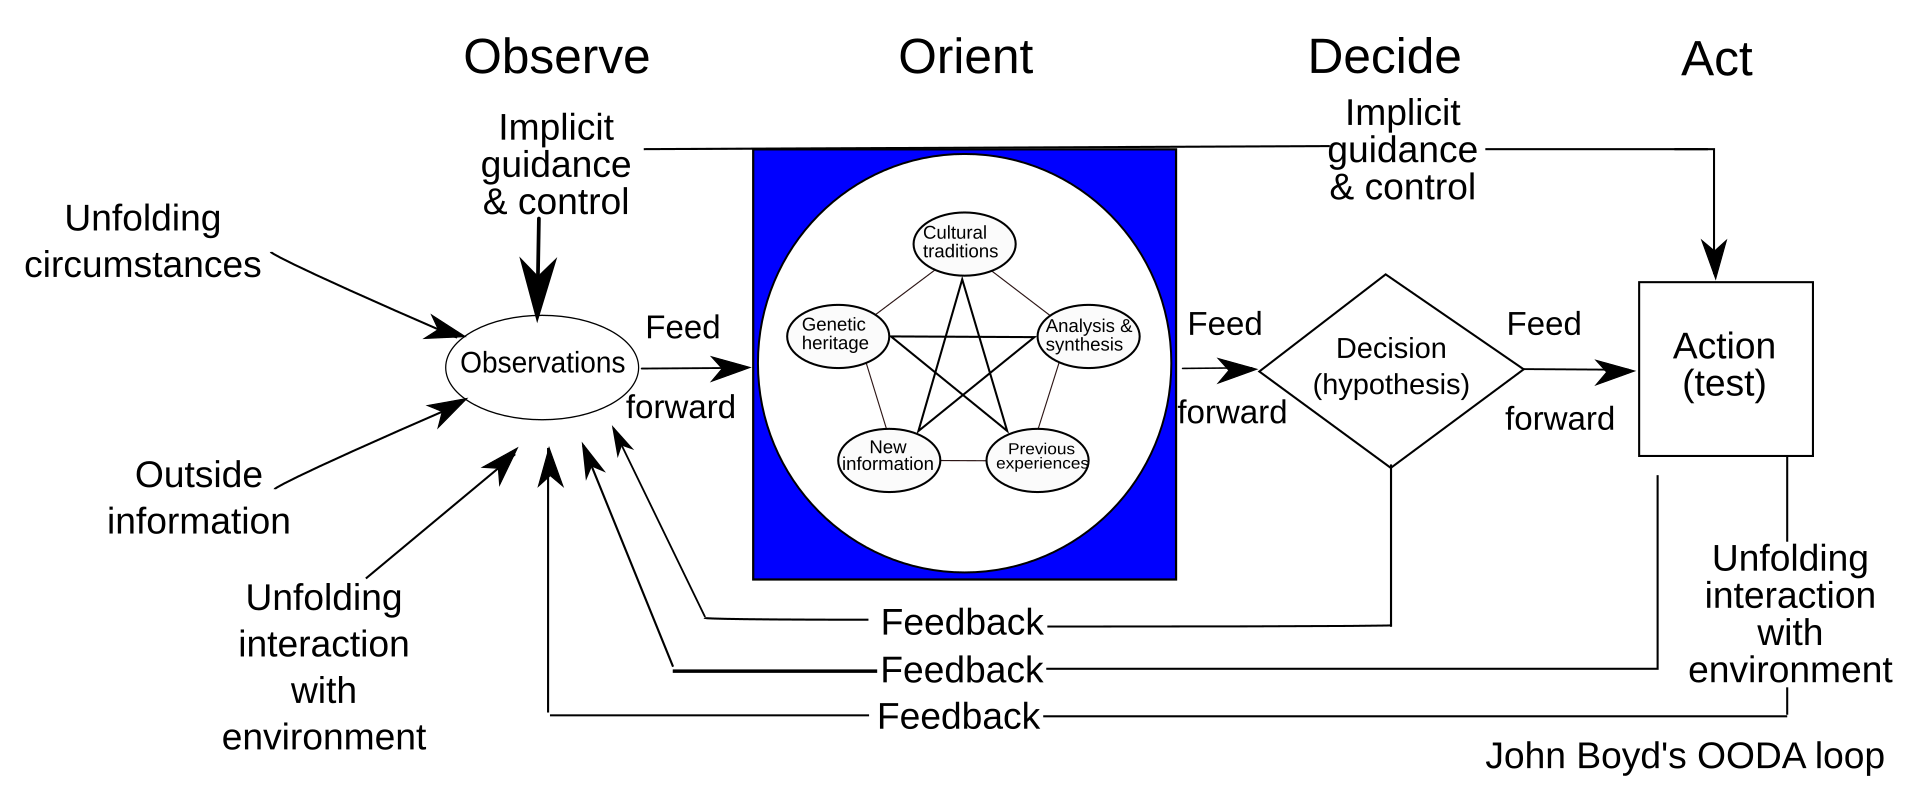
\includegraphics[width=1\linewidth]{24-ooda.png}
    \caption{Architektura pętli OODA}\label{fig:24-ooda}
\end{figure}


\subsubsection{MAPE-K}
MAPE-K jest to pętla opracowana przez IBM w dziedzinie autonomicznego przetwarzania i systemów samoadaptujących się. Głowne jej etapy to Monitorowanie, Analiza, Planowanie, Wykonanie, a każdy z nich ma dostęp do wspólnej bazy wiedzy. 

\begin{figure}[!h]
    \centering 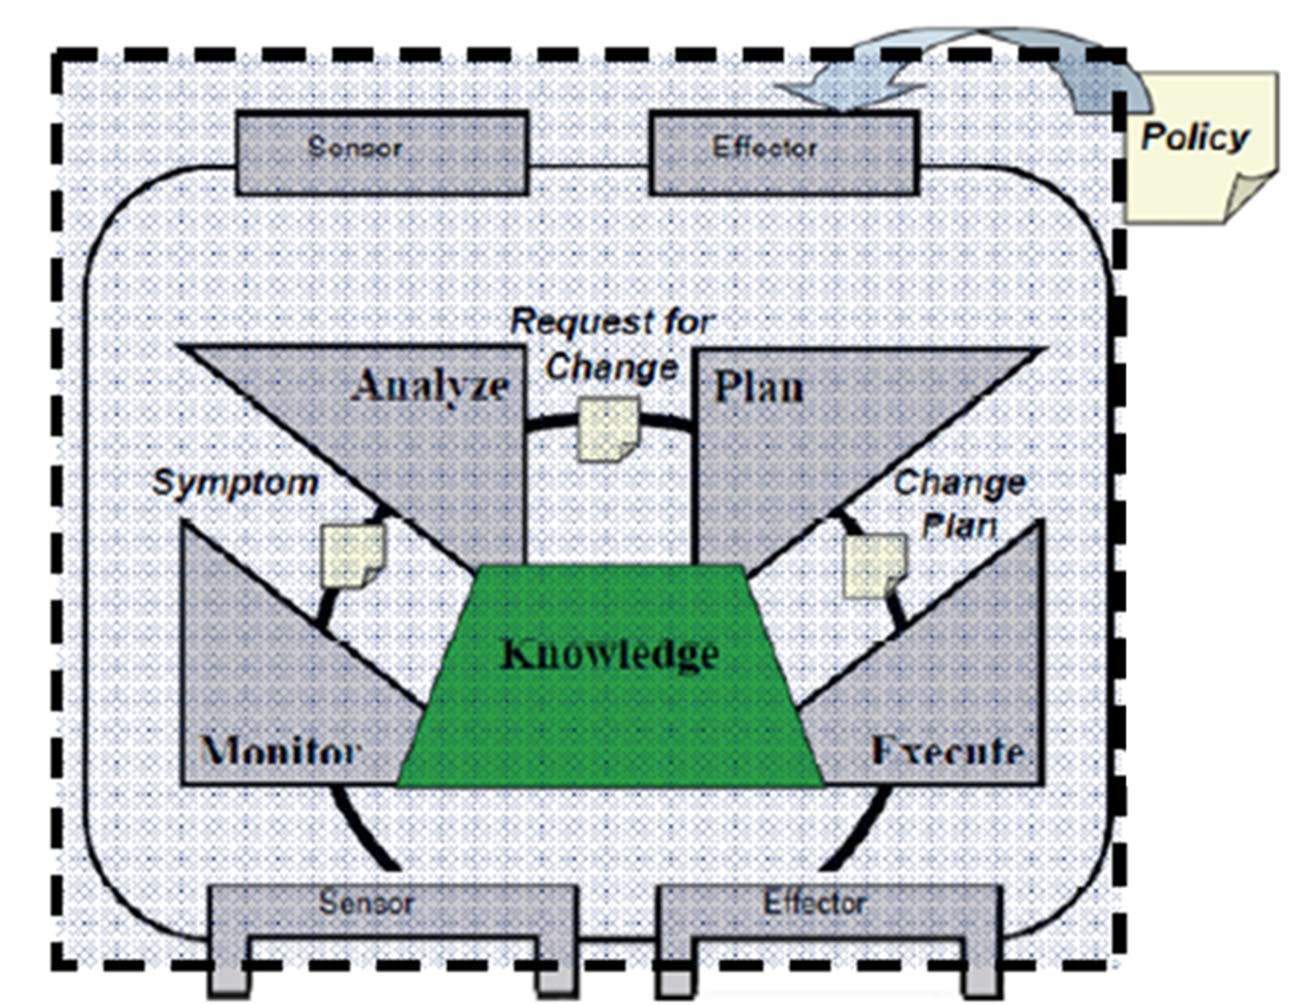
\includegraphics[width=1\linewidth]{24-mapek.png}
    \caption{Architektura pętli MAPE-K}\label{fig:24-mapek}
\end{figure}

\subsubsection{FOCALE}
Nazwa tej pętli pochodzi słów: Podstawa (ang. \textit{Foundation}), Obserwacja (ang. \textit{Observation}), Porównanie (ang. \textit{Comparison}), Analiza (ang. \textit{Analysis}), Uczenie (ang. \textit{Learning}), Wnioskowanie (ang. \textit{rEason}). Niespotykanym dotąd elementem może być Podstawa, która jest statyczną częścią modelu i określa strukturę oraz podstawowe zasady systemu. Ta architektura jako pierwsza proponuje też element odpowiedzialny za uczenie maszynowe (ang. \textit{machine learning}). 

\begin{figure}[!h]
    \centering 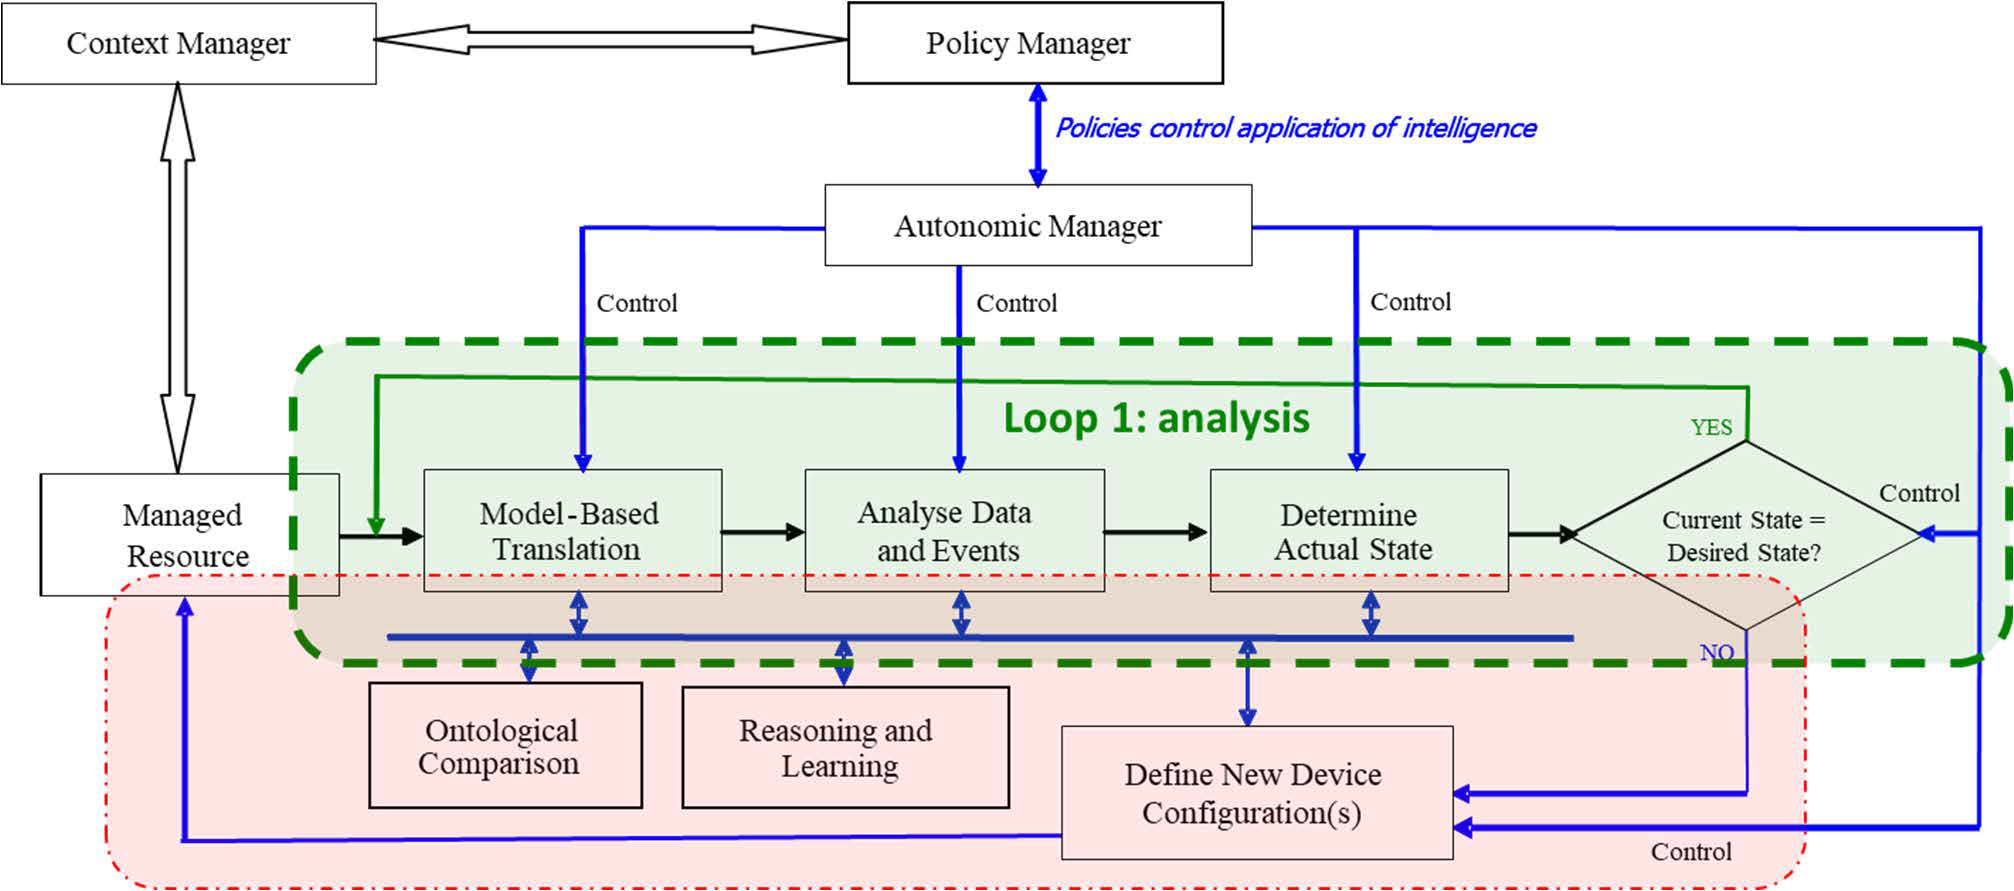
\includegraphics[width=1\linewidth]{24-focale.png}
    \caption{Architektura pętli FOCALE}\label{fig:24-focale}
\end{figure}

\subsubsection{COMPA}
Elementy tej pętli to: Analityka (ang. \textit{Analytics}), Polityki (ang. \textit{Policies}) oraz Sterowanie, Orkiestracja i Zarządzanie (ang. \text{Control, Orchestration, Management})

\begin{figure}[!h]
    \centering 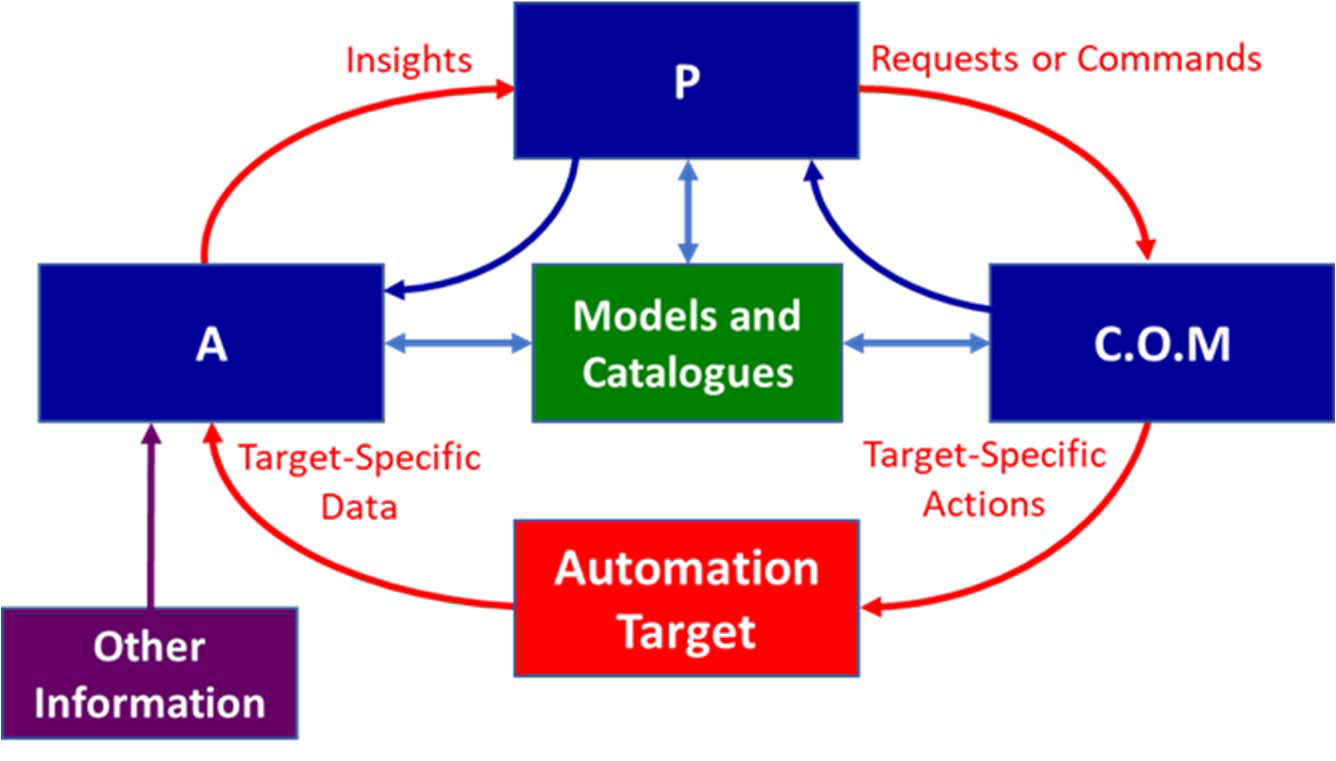
\includegraphics[width=1\linewidth]{24-compa.png}
    \caption{Architektura pętli COMPA}\label{fig:24-compa}
\end{figure}